\documentclass[a4paper]{article}
\usepackage{pdfpages}
\usepackage{fullpage} % Package to use full page
\usepackage{parskip} % Package to tweak paragraph skipping
\usepackage{tikz} % Package for drawing
\usepackage{amsmath}
\usepackage{amssymb}
\usepackage{hyperref}
\usepackage{multirow}
\usepackage{booktabs}
% \pagestyle{empty}

\usepackage{epsf}
\usepackage{pseudocode}
\usepackage{listings}
\usepackage{tikz}
\usepackage{graphicx, color}
\usepackage{amsmath}
% \usepackage{times}
% \usepackage{mathptm}

\def\O{\mathop{\smash{O}}\nolimits}
\def\o{\mathop{\smash{o}}\nolimits}
\newcommand{\e}{{\rm e}}
\newcommand{\R}{{\bf R}}
\newcommand{\Z}{{\bf Z}}

\title{Programming Assignment 3 : Number Partitioning Problem}
\author{HUIDS: 90978217 AND 90949705}
\date{04/21/2017}

\begin{document}
	
	\maketitle
	
	\section{Overview}
	In this programming assignment, we implemented a number of heuristic algorithms to solve the Number Partitioning problem. Because the Number Partitioning problem is NP-complete, heuristics must be applied to achieve solutions that are close to optimal. The heuristics that we applied were Repeated Random (randomly generating solutions and only updating with a better one), Hill climbing (generating neighbor solutions and only updating with a better solution), and Simulated annealing (generating neighbor solutions and updating sometimes with neighbors that are not better). In addition to these three heuristics, we implemented two different representations for solutions. The first is the standard representation of a solution, a sequence of positive and negative signs. This sequence partitions the problem into two groups, which are used to calculate the residue. The other representation is a pre-partitioned list. This representation consists of a list of length $n$ where each element is a number from $1$ to $n$. Indices with the same value indicate that the corresponding numbers in the problem must have the same sign.
	
	Our code may be run by executing the following commands in the terminal:
	\begin{verbatim}
	$ ./kk.py inputfile
	\end{verbatim}
	where \texttt{inputfile} specifies the file of 100 integers that represent the number partition problem for the Karmarkar-Karp algorithm to execute on.
	
	\section{Dynamic Programming}
	The dynamic programming solution to the Number partition problem involves creating an $n \times (2b+1)$ table. Every $(i,j)$ entry of the table contains a set of zero, one, or two ordered pairs, which describes the path of signs of the first $i$ numbers to make residue $j$. The ordered pairs are constructed to represent the residue from which the current element was constructed from. The first element of the ordered pair describes whether to place the $i$th number in the positive or negative set and the second element of the ordered pair describes the sequence that must have been followed to reach this signed residue. There are at most only two ordered pairs because given a particular signed residue and next number in the problem, there are only two possible signed residues that could have generated this new signed residue. For example if the current residue that is being checked is 4 and the $i$th number in the problem is 6, then the only two previous signed residues that can generate a signed residue of 4 are $-2$ and 10. Once the table is filled the optimal residue is found by looking for the smallest $k$ such that entry $(n,k)$ is nonempty. Let $A$ be the sequence that represents the number partition problem (indexed at 1). Let the table $X$ have indices $i \in [1,n]$ and $j \in [-b,b]$ . Below is the recursive definition
	\[X[i,j] = 
	\begin{cases}
	\{(+,\emptyset)\} & i = 1, j = A[1]\\
	\emptyset & i = 1, j \neq A[1] \\ 
	\emptyset & X(i-1, j + A[i]) = X(i-1, j - A[i]) = \emptyset \\
	\{(+, X[i-1, j - A[i]])\} & X(i-1, j + A[i]) = \emptyset \\
	\{(-, X[i-1, j + A[i]])\} & X(i-1, j - A[i]) = \emptyset \\
	\{(+, X[i-1, j - A[i]]), (-, X[i-1, j + A[i]])\} & otherwise
	\end{cases}`
	\]
	In essence, this recursive definition determines the residue of the next number by adding or subtracting the next number in the problem to the signed residue of the current sequence. If a residue $j$ is unattainable with the first $i$ numbers in the sequence, the value at $(i,j)$ is set to an empty set. In order to find a sign representation of this problem, the smallest $k$ such that $X[n,k]$ is found by iterating over the last row. Then the sign of one of the ordered pairs in the set is added to a list and the second element of the same ordered pair is followed to the previous row of the table. From here this process of extracting the sign of an ordered pair and following up to the next row continues until the first row is reached. The resulting list of signs will be a solution that corresponds to residue $k$. If there are multiple ways to reach a particular residue then they can also be found be tracing every possible path back through the table. 
	
	This algorithm exhaustively checks every residue that an instance of the number partition problem can make. The space complexity is $O(n(2b+1)) = O(nb)$ because there are that many elements in the table and each element has a constant upper bound of space. The runtime of this algorithm is $O(nb)$ because every entry in the table is checked exactly once and the operation done at each cell is to check two booleans.
	
	\section{Karmarkar-Karp}
	The Karmarkar-Karp algorithm can be performed in $O(n\log n)$ time if a max heap is used. Every iteration of the Karmarkar-Karp algorithm needs to find the largest two elements remaining in the problem, perform a subtraction, and push the difference onto the heap. This process is $O(\log n)$ because popping takes constant time and adding to the heap is logarithmic time. This process occurs $n-1$ times because one element is removed every iteration and the algorithm stops when there is one element remaining. Therefore the runtime of the algorithm is $O((n-1) \log n) = O(n\log n)$.
	
	\section{Results and Discussion}
	\subsection{Data}
	We generated 100 random instances of sets of 100 integers from 1 to $10^{12}$. For each instance, we first calculated the residue obtained by running KK. Then, for 25k iterations each, we ran the repeated random, hill climbing, and simulated annealing algorithms starting from a random solution and using both the standard sequence of signs and the prepartitioning representations. 
	
	After running just KK on the 100 instances, we obtained a final average residual of \textbf{222397.03}. After running the standard and prepartitioning algorithms for each instance, we obtained the following residual and time averages, included in the table below. Note that the standard sequence of signs representation's residuals are multiplied by $1E8$. If desired, see attached data file (submitted along with this PDF) for more detail. 
	
\begin{tabular}{l|ll|ll}
\textbf{}           & \multicolumn{2}{l|}{\textbf{Standard Rep.}}               & \multicolumn{2}{l|}{\textbf{Prepartitioning}} \\ \hline
\textbf{Method}     & \textbf{Avg. Residual ($\times 1e8$)} & \textbf{Time (sec)} & \textbf{Avg. Residual}  & \textbf{Time (sec)} \\ \hline
Repeated Random     & 2.97                                & 4.46                & 195.99                  & 25.87               \\
Hill Climbing       & 4.00                                & 0.86                & 709.61                  & 31.19               \\
Simulated Annealing & 2.54                                & 0.90                & 223.81                  & 27.60              
\end{tabular}
	
	\vspace{0.2in}
	The graphical representation of our data is as follows:\\\\
	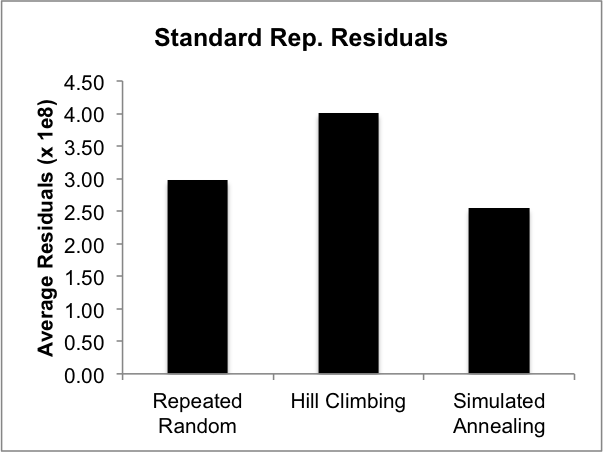
\includegraphics[width=3in]{ss_resid}
	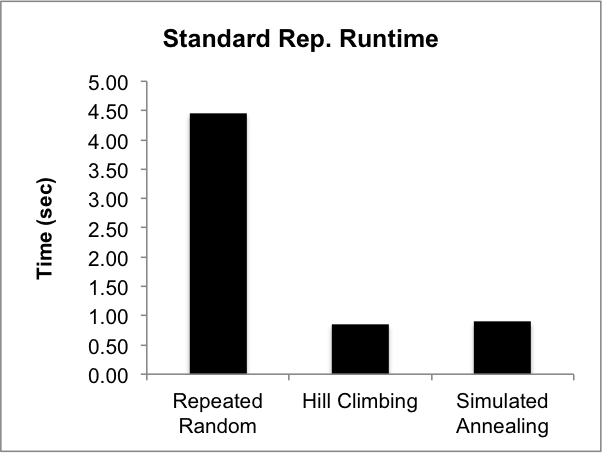
\includegraphics[width=3in]{ss_time}\\
	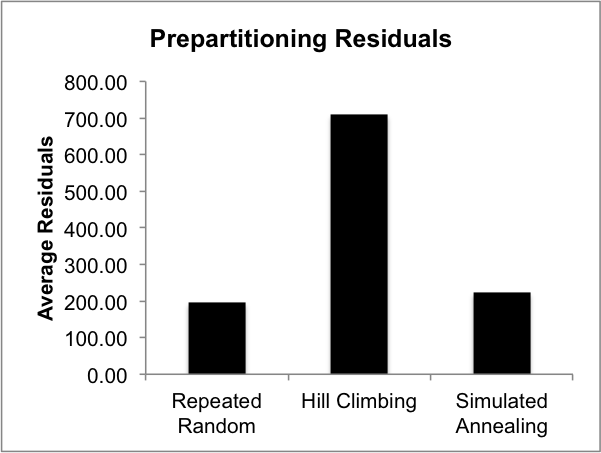
\includegraphics[width=3in]{pp_resid}
	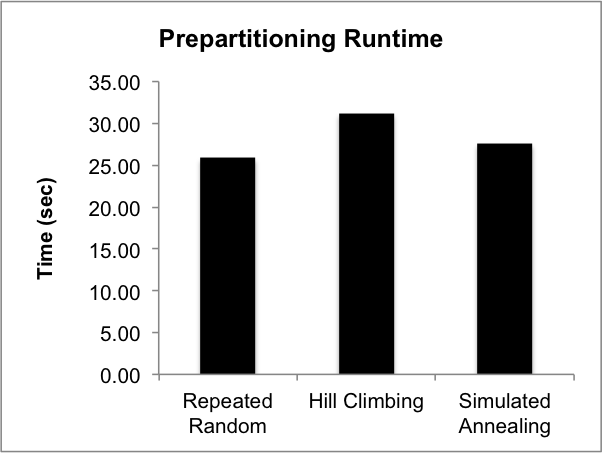
\includegraphics[width=3in]{pp_time}
	
	\subsection{Discussion}
	These data show that the prepartitioning (PP) representation is the best, followed by the single KK algorithm, followed by the standard sequence of signs (SS) representation. All three SS heuristic models returned averages with 9 digits, the single KK algorithm returned an average of 6 digits, and the prepartitioning residuals were only 3 digits. This disparity is due to the Karmarkar-Karp algorithm, which is employed in calculating the residues for PP and the single KK algorithm but not for the standard representation. Karmarkar-Karp adds another layer of heuristic that shapes the prepartitioned result to be better. Note because KK is used 25,000 times in the PP representation, as opposed to a single time for the single KK algorithm, it makes sense that PP performed the best overall. 
	
	Within one particular solution representation, hill climbing consistently performed the worst of the three heuristics. One explanation for this is that hill climbing will get stuck in local minimums. Even though a better solution can be achieved with a drastic change to the solution, hill climbing will never make this change because it will only accept marginal changes that are better. In both solution representations, simulated annealing and repeated random are relatively close in performance. Simulated annealing is not subject to the same trap of getting stuck in local minimums like hill climbing. Simulated annealing, however, is rather slow to make changes because it can only adjust to a neighbor. Repeated random makes drastic changes between iterations and only accepts better solutions. This works well for getting a good approximate answer because repeated random will not be bogged down by the way the numbers are distributed and just has a decent chance of hitting a good solution over many iterations. 
	
	The disparity in runtimes between heuristics of the same solution representation can be explained at the implementation level. Repeated random for the standard representation is slower compared to the other the other two heuristics. This is most likely due to the use of the append function when generating a random solution. Otherwise, the runtimes between heuristics are relatively close, which makes sense because many of their operations are shared with some minor constant factor differences.
	
	Comparing the runtimes of the SS and PP representations, we find that SS representation computes much faster than the PP representation. This result makes sense because of the way residue is calculated for each representation. For the SS representation, residue is calculated in $O(n)$ time because every number is just multiplied by its respective sign and summed. For the PP representation, residue is calculated in $O(n\log n)$ time because the Karmankar-Karp algorithm has to execute on the generated problem.

	
	\section{Future Work}
	
	Instead of starting our random algorithms with a random solution, we could instead start with the partitioning given by running Karmarkar-Karp algorithm on the list. Because Karmarkar-Karp always gives us a decent approximation to the ideal partitioning, we would be starting intuitively from a ``better" place than a random solution. In particular, for algorithms that involve stepping to neighbors of the initial starting list (i.e. hill climbing and simulated annealing), starting from the Karmarkar-Karp solution will be beneficial; for the repeated random method, starting from Karmarkar-Karp has no bearing on the subsequently-generated random solutions, so starting from KK likely has less benefit.
	
	Note that for all three methods, including repeated random, starting from KK ensures that the maximum residue we can obtain is our initial KK residue (i.e. we can't do worse than the initial decent solution).
	
\end{document}